%% LyX 2.3.7 created this file.  For more info, see http://www.lyx.org/.
%% Do not edit unless you really know what you are doing.
\documentclass[11pt]{article}
\renewcommand{\rmdefault}{cmr}
\renewcommand{\sfdefault}{cmss}
\usepackage{courier}
\usepackage[latin9]{inputenc}
\usepackage{geometry}
\geometry{verbose,tmargin=1in,bmargin=1in,lmargin=1in,rmargin=1in}
\usepackage{color}
\usepackage{array}
\usepackage{float}
\usepackage{url}
\usepackage{amsmath}
\usepackage{graphicx}
\usepackage[unicode=true,
 bookmarks=false,
 breaklinks=false,pdfborder={0 0 1},backref=section,colorlinks=true]
 {hyperref}
\hypersetup{
 linkcolor=blue,urlcolor=blue,filecolor=blue}

\makeatletter

%%%%%%%%%%%%%%%%%%%%%%%%%%%%%% LyX specific LaTeX commands.
\providecommand{\LyX}{\texorpdfstring%
  {L\kern-.1667em\lower.25em\hbox{Y}\kern-.125emX\@}
  {LyX}}
%% Because html converters don't know tabularnewline
\providecommand{\tabularnewline}{\\}

%%%%%%%%%%%%%%%%%%%%%%%%%%%%%% Textclass specific LaTeX commands.
\providecommand*{\code}[1]{\texttt{#1}}

%%%%%%%%%%%%%%%%%%%%%%%%%%%%%% User specified LaTeX commands.
\usepackage{listings}
\lstset{
  language={C++},
  frame=tb,
  numbers=left,
  numberstyle=\tiny,
  basicstyle=\small\sffamily,
  breaklines=true,
}

\makeatother

\usepackage{listings}
\renewcommand{\lstlistingname}{Listing}

\begin{document}
\begin{center}
\textbf{\Large{}CSCE 221 Cover Page} \\
 \medskip{}
\par\end{center}

Please list all sources in the table below including web pages which
you used to solve or implement the current homework. If you fail to
cite sources you can get a lower number of points or even zero, read
more Aggie Honor System Office \url{https://aggiehonor.tamu.edu/}
\\

\noindent \begin{center}
{\large{}}%
\begin{tabular}{|>{\raggedright}p{0.2\linewidth}|p{0.45\linewidth}|}
\hline 
\noalign{\vskip\doublerulesep}
{\large{}Name } & {\large{}Tianlan Li }\tabularnewline[\doublerulesep]
\hline 
\noalign{\vskip\doublerulesep}
{\large{}UIN } & {\large{}532003637 }\tabularnewline[\doublerulesep]
\hline 
\noalign{\vskip\doublerulesep}
{\large{}Email address } & {\large{}rainsuds@tamu.edu }\tabularnewline[\doublerulesep]
\hline 
\end{tabular} 
\par\end{center}

Cite your sources using the table below. Interactions with TAs and
resources presented in lecture do not have to be cited. 
\noindent \begin{center}
{\large{}}%
\begin{tabular}{|>{\centering\arraybackslash}m{0.25\linewidth}|>{\raggedright}m{0.7\textwidth}|}
\hline 
\noalign{\vskip\doublerulesep}
{\large{}People } & \begin{enumerate}
\item {\large{}None }
\end{enumerate}
\tabularnewline[\doublerulesep]
\hline 
\noalign{\vskip\doublerulesep}
{\large{}Webpages } & \begin{enumerate}
\item {\large{}Mapping 2-3-4 Trees into Red-Black Trees. Mapping 2-3-4 trees into red-black trees. (n.d.). https://azrael.digipen.edu/~mmead/www/Courses/CS280/Trees-Mapping2-3-4IntoRB.html  }
\end{enumerate}
\tabularnewline[\doublerulesep]
\hline 
\noalign{\vskip\doublerulesep}
{\large{}Printed Materials } & \begin{enumerate}
\item {\large{}None }
\end{enumerate}
\tabularnewline[\doublerulesep]
\hline 
\noalign{\vskip\doublerulesep}
{\large{}Other Sources } & \begin{enumerate}
\item {\large{}None }
\end{enumerate}
\tabularnewline[\doublerulesep]
\hline 
\end{tabular} 
\par\end{center}

\pagebreak{}
\begin{center}
\textbf{\Huge{}Homework 2}{\Huge\par}
\par\end{center}

\begin{center}
\bigskip{}
\textbf{\Large{}Due date is on the Canvas calendar} 
\par\end{center}

\noindent \begin{flushleft}
\textbf{Typeset your solutions to the homework problems preferably
in \LaTeX{} or \LyX . See the class webpage for information about their
installation and tutorials. There are 7 problems on 7 separate pages.}
\par\end{flushleft}
\begin{enumerate}
\item (15 points) Provided two sorted lists, \texttt{l1} and \texttt{l2},
write a function in C++ to \emph{efficiently} compute \texttt{$\mathtt{l1\cap l2}$}
using only the basic STL list operations. The lists may be empty or
contain a different number of elements e.g. $\mathtt{|l1|}\neq\mathtt{|}\mathtt{l2|}$
You may assume \texttt{l1} and \texttt{l2} will not contain duplicate
elements. 

\noindent Examples (all set members are list node): 
\begin{itemize}
\item $\{1,2,3,4\}\cap\{2,3\}=\{2,3\}$ 
\item $\emptyset\cap\{2,3\}=\emptyset$ 
\item $\{2,9,14\}\cap\{1,7,15\}=\emptyset$ 
\end{itemize}
\bigskip{}

\begin{enumerate}
\item Complete the function below. Do not use any routines from the algorithm
header file.

\begin{lstlisting}[language={C++},basicstyle={\small\ttfamily},tabsize=4]
#include <list>

std::list<int> intersection(const std::list<int>& l1, 
                            const std::list<int>& l2) {
  std::list<int> ans;
    auto it1 = l1.begin();
    auto it2 = l2.begin();

    while (it1 != l1.end() && it2 != l2.end()) {
        if (*it1 < *it2) {
            ++it1;
        }
        else if (*it1 > *it2) {
            ++it2;
        }
        else {
            ans.push_back(*it1);
            ++it1;
            ++it2;
        }
    }
    return ans;
}
\end{lstlisting}

\item Verify that your implementation works properly by writing two test
cases.

\item[\textbf{Solution:}]  
Test case 1:\\
l1 = $\{2, 4, 6, 8, 10\}$\\
l2 = $\{2, 6, 10\}$\\

Excepted output:\\
$\{2, 6, 10\}$\\
Actual output:\\
$\{2, 6, 10\}$\\

Test case 2:\\
l1 = $\{\}$\\
l2 = $\{1, 2, 3\}$\\

Excepted output:\\
$\{\}$\\
Actual output:\\
$\{\}$\\

\item What is the running time of your algorithm? Provide a big-O bound.
Justify.

\item[\textbf{Solution:}]
The running time of my algorithm is O(n) where n is the total input size of both list. Since the while loop must travels through the entirety of both list, the worst-case running time of this function would be size of l1 plus size of l2.

\pagebreak{}
\end{enumerate}
\item (15 points) Write a C++ recursive function that counts the number
of nodes in a singly linked list. Do not modify the list. 

Examples: 
\begin{itemize}
\item \code{count\_nodes($(2)\rightarrow(4)\rightarrow(3)\rightarrow\text{nullptr}$)}
= 3 
\item \code{count\_nodes($\text{nullptr}$)} = 0 
\end{itemize}
\bigskip{}

\begin{enumerate}
\item Complete the function below: \label{enum:recursive_node_imp}

\begin{lstlisting}[language={C++},basicstyle={\small\ttfamily},tabsize=4]
template<typename T>
struct Node {
  Node* next;
  T obj;

  Node(T obj, Node* next = nullptr)
    : obj(obj), next(next)
  { }
};

template<typename T>
int count_nodes(Node<T>* node) {
    // Insert code
    if (node == nullptr) {
        return 0;
    }
    return 1 + count_nodes(node->next);
}
\end{lstlisting}

\item Verify that your implementation works properly by writing two test
cases for the function you completed in part \ref{enum:recursive_node_imp}.

\item[\textbf{Solution:}]
Test case 1:\\
l1 = $(2)->(4)->(3)->nullptr$

Excepted output:\\
3\\
Actual output:\\
3\\

Test case 2:\\
l2 = nullptr\\

Excepted output:\\
0\\
Actual output:\\
0
 
\item Write a recurrence relation that represents your algorithm.

\item[\textbf{Solution:}]
T(n) = T(n - 1) + O(1)

\item Solve the recurrence relation using the iterating or recursive tree
method to obtain the running time of the algorithm in Big-O notation.

\item[\textbf{Solution:}]
To solve the recurrence relation:
\[T(n) = T(n-1) + O(1)\]

Expanding the relation:
\begin{align*}
T(n) & = T(n-1) + O(1) \\
     & = (T(n-2) + O(1)) + O(1) \\
     & = T(n-2) + 2O(1) \\
     & = T(n-3) + 3O(1) \\
     & \ldots \\
     & = T(n-k) + kO(1)
\end{align*}

Consider $n-k = 0$, which means $k = n$. In this case:
\[T(n-n) + nO(1) = T(0) + nO(1)\]
Since $T(0)$ is a constant time operation, so the running-time function of the recursive algorithm is $O(n)$.
\[T(n) = O(1) + nO(1) = O(1) + O(n) = O(n)\]

Therefore, the running time of the algorithm in Big-O notation is $O(n)$. The \texttt{count\_nodes} algorithm has a linear time complexity, which means the time it takes to count the nodes in a singly linked list is directly proportional to the number of nodes in the list.

\end{enumerate}
\pagebreak{}
\item (15 points) Write a C++ recursive function that finds the maximum
value in an array (or vector) of integers \emph{without} using any
loops. You may assume the array will always contain at least one integer.
Do not modify the array. 
\begin{enumerate}
\item Complete the function below:

\begin{lstlisting}[language={C++},basicstyle={\small\ttfamily},tabsize=4]
#include <vector>

int find_max_value(std::vector<int> vec, int start, int end) {
	// Insert code
    if (start == end) {
        return vec[start];
    }
    else {
        int mid = (start + end) / 2;
        int max_left = find_max_value(vec, start, mid);
        int max_right = find_max_value(vec, mid + 1, end);
        return (max_left > max_right) ? max_left : max_right;
    }
}
\end{lstlisting}

\item Verify that your implementation works properly by writing two test
cases.

\item[\textbf{Solution:}]
Test case 1:\\
v1 = $\{1, 2, 3, 4, 5, 6, 7, 8\}$

Excepted output:\\
8\\
Actual output:\\
8\\

Test case 2:\\
v2 = $\{2, 10, 11, 22, 100, 1, 4\}$\\

Excepted output:\\
100\\
Actual output:\\
100

\item Write a recurrence relation that represents your algorithm.

\item[\textbf{Solution:}]
$T(n) = 2T(\frac{n}{2}) + O(1)$

\item Solve the recurrence relation and obtain the running time of the algorithm
in Big-O notation. Show your process.

\item[\textbf{Solution:}]
According the to Master Theorem, $T(n) = aT(\frac{n}{b}) + f(n)$ where $a = 2$, $b = 2$, and $f(n) = O(1)$. Comparing $f(n)$ to $n^{log_b(a)}$, which is $n^{log_2 (2)} = n^1$, and $f(n) = O(1)$, since constant running time is negligible in larger input of $n$. Therefore the running time of the algorithm is $O(n)$.


\pagebreak{}
\end{enumerate}
\item (15 points) What is the best, worst and average running time of quick
sort algorithm? 
\begin{enumerate}
\item Provide recurrence relations. For the average case, you may assume
that quick sort partitions the input into two halves proportional
to $c$ and $1-c$ on each iteration. \label{enum:recurrence_relation}

\item[\textbf{Solution:}]
Best case: $T(n) = 2T(n/2) + O(n)$\\
Average case: $T(n) = T(nc) + T(n(1-c)) + O(n)$\\
Worst case: $T(n) = T((n-1)/n) + T(n(1-((n-1)/n))) + O(n)$

\item Solve each recurrence relation you provided in part \ref{enum:recurrence_relation}

\item[\textbf{Solution:}]
Best Case:\\
The best-case time complexity of quicksort is given by the recurrence relation:
\[T(n) = 2T\left(\frac{n}{2}\right) + O(n)\]
By applying the Master Theorem, where $a = 2$ and $b = 2$, and noting that $f(n) = O(n)$, we can conclude that $T(n) = \Theta(n \log n)$. Therefore, the best-case time complexity is $\Theta(n \log n)$.\\

Average Case:\\
The average-case time complexity analysis for quicksort considers the expected behavior of the algorithm when the pivot divides the array into two roughly equal halves on average. While the analysis is probabilistic, it often results in an expected time complexity of $O(n \log n)$, which is the same as the best-case scenario.\\

Worst Case:\\
\[T(n) = T((n-1)/n) + T(n(1-((n-1)/n))) + O(n)\]
\[T(n) = T(\frac{n-1}{n})+ T(1) + O(n)\]
In the worst case, quick sort exhibits a time complexity of $O(n^2)$. This occurs when the pivot selection consistently results in highly unbalanced partitions, leading to a recurrence relation with an approximate height of $n$. The array size after each iteration is approximately $1 + (n - 1)$, contributing to the worst-case running time of $O(n^2)$.

\item Provide an arrangement of the input array which results in each case.
Assume the first item is always chosen as the pivot for each iteration.

\item[\textbf{Solution:}]
Best Case:\\
$[5, 2, 3, 4, 1, 6, 7, 8, 9, 10]$\\

Average Case:\\
$[5, 3, 8, 2, 7, 1, 10, 4, 9, 6]$\\

Worst Case:\\
$[10, 9, 8, 7, 6, 5, 4, 3, 2, 1]$\\

\end{enumerate}
\pagebreak{}
\item (15 points) Write a C++ function that counts the total number of nodes
with two children in a binary tree (do not count nodes with one or
none child). You can use a STL container if you need to use an additional
data structure to solve this problem. 
\begin{figure}[H]
\centering{}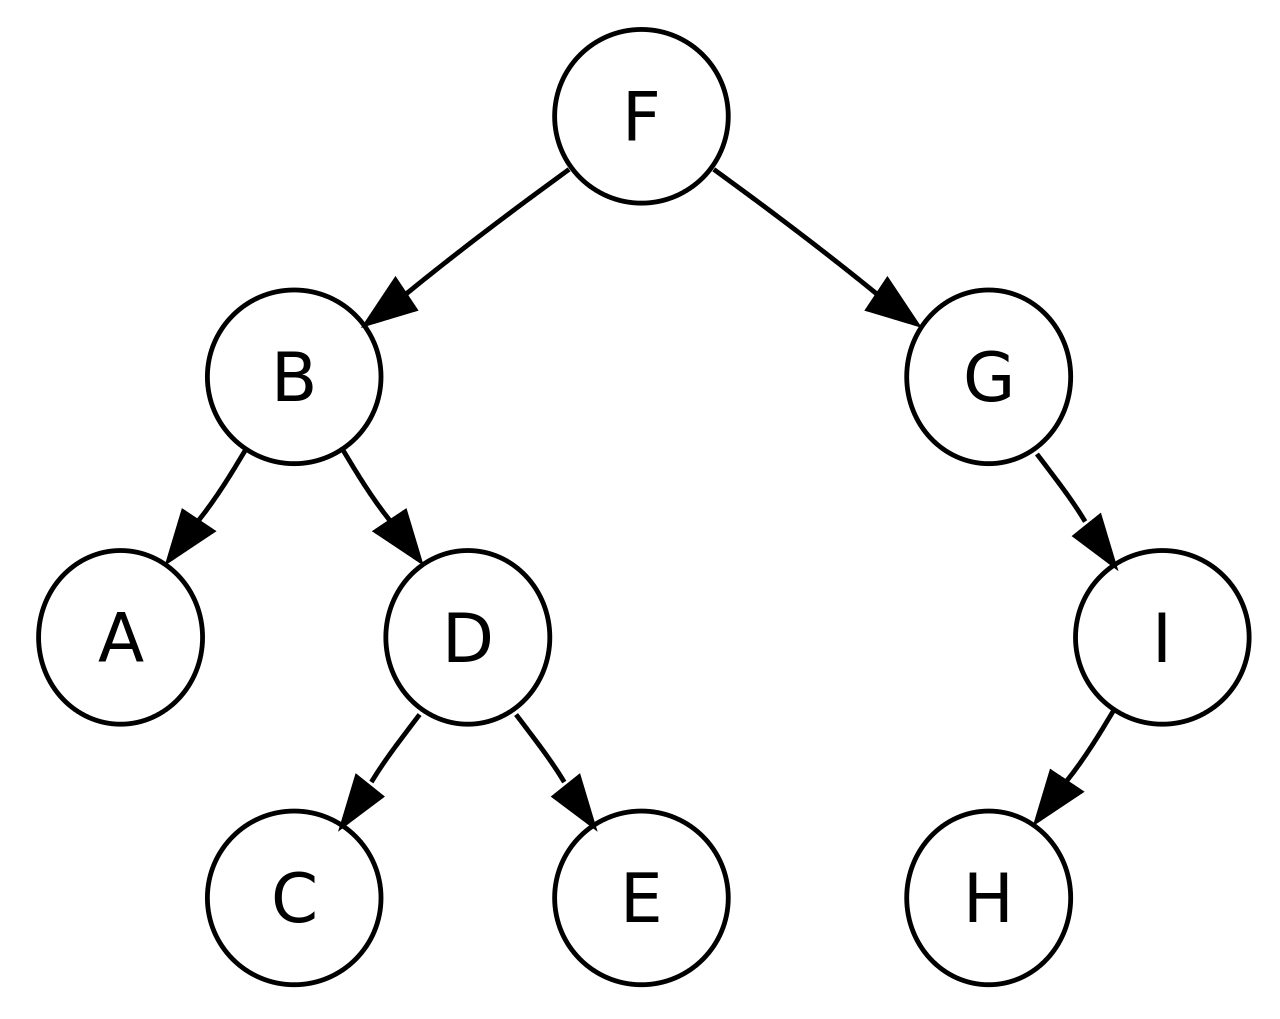
\includegraphics[width=0.3\linewidth]{binary_tree_example}
\caption{Calling \protect\code{count\_filled\_nodes} on the root node F returns
\protect\code{3}}
\label{fig:binary_tree_example} 
\end{figure}

\begin{enumerate}
\item Complete the function below. The function will be called with the
root node (e.g. \code{count\_filled\_nodes(root)}). The tree may
be empty. Do not modify the tree.

\begin{lstlisting}[language={C++},basicstyle={\small\ttfamily},tabsize=4]
#include <vector>

template<typename T>
struct Node {
  Node<T>* left;
  Node<T>* right;
  T obj;

  Node(T o, Node<T>* l = nullptr, Node<T>* r = nullptr)
    : obj(o), left(l), right(r)
  { }
};

template<typename T>
int count_filled_nodes(const Node<T>* node) {
	// Insert code
    if (node == nullptr) {
        return 0;
    }
    int count = 0;
    if (node->left != nullptr && node->right != nullptr) {
        count = 1;
    }
    count += count_filled_nodes(node->left);
    count += count_filled_nodes(node->right);

    return count;
}
\end{lstlisting}

\item Use big-O notation to classify your algorithm. Show how you arrived
at your answer.

\item[\textbf{Solution:}]
The algorithm can be written as T(n) = 2(n/2) + O(1), by the master theorem, which simplifies down to T(n) = O(n). The function travels to each node exactly once by calling the left subtree and right subtree recursively.

\end{enumerate}
\pagebreak{}
\item (15 points) For the following statements about red-black trees, provide
a justification for each true statement and a counterexample for each
false one. 
\begin{enumerate}
\item A subtree of a red-black tree is itself a red-black tree.

\item[\textbf{Solution:}]
False, the root of a red-black tree must be black, therefore any subtree with a red root node is nota red-black tree.

\item The sibling of an external node is either external or red.

\item[\textbf{Solution:}]
False, the sibiling of a external node can be another black node with value, a NIL node, or a red node.

\item There is a unique 2-4 tree associated with a given red-black tree.

\item[\textbf{Solution:}]
True, A 2-4 tree 2-node requires one red/black node, a 3-node requires two red/black nodes, and a 4-node requires 3 red/black nodes. The data structures are isomorphic to each other.


\item There is a unique red-black tree associated with a given 2-4 tree.

\item[\textbf{Solution:}]
True, A black node that started out with two black children will still have two black children after this transformation. A black node that started out with one red and one black child will have three children after this transformation. A black node that started out with two red children will have four children after this transformation. 
\end{enumerate}
\pagebreak{}
\item (10 points) Modify this skip list after performing the following series
of operations: \code{erase(38)}, \code{insert(48,x)}, \code{insert(24,y)},
\code{erase(42)}. Provide the recorded coin flips for \code{x} and
\code{y}. 

\begin{tabular}{ccccccccccccc}
$-\infty$  &  & -----  &  & -----  &  & -----  &  & -----  &  & -----  &  & $+\infty$\tabularnewline
 &  &  &  &  &  &  &  &  &  &  &  & \tabularnewline
$-\infty$  &  & -----  &  & 17  &  & -----  &  & -----  &  & -----  &  & $+\infty$\tabularnewline
 &  &  &  &  &  &  &  &  &  &  &  & \tabularnewline
$-\infty$  &  & -----  &  & 17  &  & -----  &  & -----  &  & ----  &  & $+\infty$\tabularnewline
 &  &  &  &  &  &  &  &  &  &  &  & \tabularnewline
$-\infty$  &  & -----  &  & 17  &  & -----  &  & 24  &  & ----  &  & $+\infty$\tabularnewline
 &  &  &  &  &  &  &  &  &  &  &  & \tabularnewline
$-\infty$  &  & 12  &  & 17  &  & -----  &  &  24 &  & 48  &  & $+\infty$\tabularnewline
 &  &  &  &  &  &  &  &  &  &  &  & \tabularnewline
$-\infty$  &  & 12  &  & 17  &  & 20  &  & 24  &  & 48  &  & $+\infty$\tabularnewline
\end{tabular}\bigskip{}

\textbf{x:} TH
\textbf{y:} TTH 
\end{enumerate}

\end{document}
